%
%%%%%%%%%%%%%%%%%%%%%%%%%%%%%%%%%%%%%%%%%%%%%%%%%%%%%%%%%%%%%%%%%%%%%%
% Tina Dissertation
% December 2013, modified to Template June 2015
%%%%%%%%%%%%%%%%%%%%%%%%%%%%%%%%%%%%%%%%%%%%%%%%%%%%%%%%%%%%%%%%%%%%%%
% Documentclass Memoir 
% check memman.pdf for help and information
%%%%%%%%%%%%%%%%%%%%%%%%%%%%%%%%%%%%%%%%%%%%%%%%%%%%%%%%%%%%%%%%%%%%%%
\documentclass[openright,12pt,a4paper]{memoir} 
\usepackage{graphicx}
%\usepackage[utf8]{inputenc} % set input encoding to utf8
\usepackage{array} % for tables 
\usepackage{multirow} % for tables 
\usepackage{multicol} % for tables
\usepackage{tabularx} % for tables
\usepackage{booktabs}
\usepackage{cite}
\usepackage{tabularx}
\usepackage[round]{natbib}
\usepackage{threeparttable}
\DisemulatePackage{setspace}
\usepackage{setspace}
\usepackage{longtable}
\usepackage{tabu}
\usepackage{pdflscape}
\usepackage{caption}
%\usepackage{lmodern}
\usepackage{url} \usepackage[normalem]{ulem}
\useunder{\uline}{\ul}{}



% defines new column type
\newcolumntype{Z}{$>${\raggedright\arraybackslash}X}

% add a little vertical padding to cramped tables
\setlength{\extrarowheight}{2pt}


%%%%%%%%%%%%%%%%%%%%%%%%%%%%%%%%%%%%%%%%%%%%%%%%%%%%%%%%%%%%%%%%%%
%%% Examples of Memoir customization
%%% enable, disable or adjust these as desired

%%% PAGE DIMENSIONS
% a4paper is by default 210mm wide and 279 mm wide

% default document in memoir is twoside (recto-verso) and openright (new chapter begins on recto page)

% size of the text area
  \settrims{0pt}{0pt}
  \settypeblocksize{230mm}{147mm}{*}
  \setlength{\spinemargin}{27mm}
  \setlength{\foremargin}{36mm}
%\setulmargins{35mm}{45mm}{*}
%\setlength{\marginparwidth}{0mm}
%\setlength{\marginparsep}{0mm}
%\setlength{\textwidth}{140mm}
%\settrimmedsize{0.9\stockheight}{0.9\stockwidth}{*}
%\setlength{\trimtop}{0pt}
%\setlength{\trimedge}{0pt}
%\addtolength{\trimedge}{-\paperwidth}
%\settypeblocksize{*}{\lxvchars}{1.618} % we want to the text block to have golden proportionals
  \setulmargins{*}{*}{1.618} % 50pt upper margins
%\setlrmargins{*}{*}{1.3}
%  \setlrmargins{*}{*}{1} % golden ratio again for left/right margins
  \setheaderspaces{*}{*}{1.618}
  \checkandfixthelayout % to make sure that the layout parameters make sense

%\addtolength{\textwidth}{0cm}
%\addtolength{\textheight}{1.5cm}
%\addtolength{\textwidth}{-2cm}
%\addtolength{\textheight}{+0.5cm}

%%% \maketitle CUSTOMISATION
% For more than trivial changes, you may as well do it yourself in a titlepage environment
%\pretitle{\begin{center}\sffamily\Huge\MakeUppercase}
%\posttitle{\par\end{center}\vskip 0.5em}

%%% ToC (table of contents) APPEARANCE
  \maxtocdepth{subsection} % include subsections
%\renewcommand{\cftchapterpagefont}{}
%\renewcommand{\cftchapterfont}{}     % no bold!

%%% HEADERS & FOOTERS
  \pagestyle{headings} % try also: empty , plain , headings , ruled , Ruled , companion

%%% CHAPTERS
  \chapterstyle{southall} % try also: default , section , hangnum , companion , article, demo

  \renewcommand{\chaptitlefont}{\LARGE\sffamily\raggedright} % set sans serif chapter title font
  \renewcommand{\chapnumfont}{\LARGE\sffamily\raggedright} % set sans serif chapter number font

%%% TABLES
  \newcolumntype{C}[1]{$>${\centering}m{#1}} % defines the default layout of the tables (C$=$centerling, L$=$left)
  \newcolumntype{L}[1]{$>${\centering}m{#1}}

%%% SECTIONS
%\hangsecnum % hang the section numbers into the margin to match \chapterstyle{hangnum}
  \maxsecnumdepth{section} % number subsections

  \setsecheadstyle{\Large\sffamily\raggedright} % set sans serif section font
  \setsubsecheadstyle{\large\sffamily\raggedright} % set sans serif subsection font

%%% Abstract
  \setlength{\absleftindent}{0mm}
  \setlength{\absrightindent}{0mm}

  \renewcommand{\absnamepos}{center}
  \setlength{\abstitleskip}{+0cm}

%%% Captions

%\DeclareCaptionFont{tiny}{\tiny}
%\captionsetup{font$=$tiny, labelfont$=$tiny}
%\usepackage[font$=${tiny}, labelfont$=${tiny}]{caption}
%\usepackage[font$=$sf, labelfont$=${sf,bf}, margin$=$1cm]{caption}
%\captionsetup{font$=$scriptsize,labelfont$=$scriptsize}

%\usepackage[textfont$=${tiny}, labelfont$=${tiny}]{caption}

 % \captionnamefont{\tiny}
 %\captiontitlefont{\tiny}

%% END Memoir customization


%%%%%%%%%%%%%%%%%%%%%%%%%%%%%%%%%%%%%%%%%%%%%%%%%%%%%%%%%%%%%%%%%%%%%%%%%%%%%%%%%%%%%%%%%%%%%%%%%%%%%%%%%%%%%%%%%%%%%%%%%%%%%%%%%%%%%%%%%%%%%
%%% BEGIN DOCUMENT

\begin{document}
\doublespacing


\chapter[functional diversity]{Heterogeneous flows foster heterogeneous assemblages: relationships between functional diversity and hydrological heterogeneity in riparian plant communities}
\newpage

\section*{Abstract}
Riparian ecosystems are biophysically complex and highly diverse taxonomically, structurally and functionally. While many environmental factors determine the structure and function of riparian vegetation communities, hydrology is thought to be the ‘master variable’. Flooding and variability in water availability are known to be key drivers of taxonomic diversity, but their influence on the functional trait diversity of riparian vegetation communities remains largely unexplored.

We collected data on species abundance, quantitative plant functional traits and hydrology from 15 sites distributed across south-eastern Australia to address the following questions: (a) is functional trait diversity related to frequency and magnitude of flooding disturbance? (b) is functional trait diversity related to variability in seasonal water availability within the riparian zone?

We confirm that metrics describing both flooding disturbance and patterns of water availability exhibit strong relationships with functional trait diversity in riparian vegetation communities of south-eastern Australia. Our key finding is that functional trait diversity in these systems tends to be positively associated with variability in hydrological conditions and the intensity of rare, high magnitude flooding events, rather than average patterns of flow.

Our study highlights the importance of extreme flooding events and temporal patterns of water availability as determinants of diversity in riparian vegetation communities. These relationships may have significant consequences for plant communities experiencing alterations to hydrology caused by anthropogenic flow modification and the changing climate. 

\section*{Keywords}
riparian vegetation, functional trait, functional diversity, environmental heterogeneity, disturbance

\clearpage

\section{Introduction}
Riparian ecosystems are biophysically complex and highly diverse taxonomically, structurally and functionally \cite{Naiman1993, Poff2002, Nilsson2002}. Extensive flow regulation of river systems and changing patterns of runoff under future climates are likely to produce dramatically different future flow regimes, with significant consequences for the diversity and functioning of riparian assemblages. Riverine conservation and rehabilitation efforts must therefore be informed by general understanding of the processes that generate patterns of diversity and drive ecosystem functioning in riparian ecosystems.

The prevailing paradigm in riparian ecology holds that heterogeneity in the riparian patch mosaic results from the sculpting action of hydrological processes across the biogeomorphic template \cite{Tabacchi1996, Palmer1997, Corenblit2007, Bornette2008}. In riparian environments, it is this intrinsic environmental heterogeneity that fosters structural, taxonomic and functional heterogeneity within vegetation communities \cite{Naiman1993, Corenblit2007, Bornette2008}. Local hydrology (river flow regime) is widely considered to be the most important determinant of community composition and functioning in riparian plant assemblages, as it dictates patterns of disturbance by flooding, as well as soil moisture availability \cite{Poff1997, Arthington2010}.

Flooding may retard competitive exclusion by resetting the patch structure of parts of the landscape and thereby enhance diversity \cite{Huston1979, Naiman1993}, or constrain assemblages to species that have ecological strategies adapted to flooding, thereby decreasing diversity \cite{Diaz1998}. General support has been found for the intermediate disturbance hypothesis \cite{connell1978diversity} with respect to the relationship between flooding intensity and taxonomic diversity (e.g. \cite{Bendix1997, Bendix2000, Lite2005, Corenblit2007}. This support is not equivocal however \cite{Nilsson1989, Baker1990} and at within-reach scales the geomorphic template is also a strong control on diversity \cite{Bendix1997, ODonnell2014}.
 
In regions where riparian plants experience periodic water stress, soil moisture availability may be driven largely by hydrology \cite{Castelli2000, Nilsson2002}. Seasonal and interannual variability in patterns of disturbance and water availability are also known to influence species richness \cite{Greet2011, Catford2012, Catford2014} and this effect may be exacerbated for summer flows in hot or dry regions \cite{Garssen2014}. A study investigating drivers of riparian vegetation community structure and composition in subtropical eastern Australia identified variability in dry season flows as the hydrological variable that was most strongly associated with variation in species richness \cite{Arthingon2012}.
 
Conservation and restoration activities increasingly aim to preserve the ecosystem functions associated with biological communities \cite{Aerts2011, Cadotte2011, Montoya2012}. Quantitative functional traits (such as specific leaf area, wood density, seed mass, etc.) can form the basis for mechanistic assessments of diversity that describe the range and distribution of ecological strategies in a community and their associated environmental effects. Such metrics of functional trait diversity (hereafter referred to as ‘functional diversity’) are substantially more powerful than taxonomic metrics as indicators of ecosystem functioning, ecosystem resilience and capacity to provide ecosystem services \cite{Tilman1997, Diaz2001, Hooper2005}. Reduced abundance of functionally unique species may gradually undermine ecosystem resilience or functioning, and assessment of functional diversity can be useful to diagnose degradation before species loss occurs \cite{Mouillot2013}. Assessments of ecosystem service production have also begun to give functional diversity priority over taxonomic metrics \cite{Diaz2007}.
 
Numerous metrics of functional diversity have been described in the literature \cite{Schleuter2010, Mouillot2013}. These aim to quantify "the distribution of species and their abundances in the functional space of a given community” \cite{Mouillot2013}(page 167) and typically process multidimensional trait data to output a single value describing various properties of these data. The framework described by Villéger, Mason & Mouillot \cite{Villeger2008}, consisting of functional richness (the volume of the convex hull circumscribing the range of trait values), functional divergence (divergence in the distribution of abundance within trait space) and functional evenness (the evenness of this distribution in trait space), has been commonly used to describe functional diversity (e.g. \cite{Biswas2010, Pakeman2011, Savage2012, Clark2012}). Functional dispersion (FDis), defined as the abundance-weighted mean distance in multivariate trait space of individual species to the centroid of all species in the community, represents an improvement on this framework \cite{Laliberte2010}. FDis allows for consideration of species’ abundances while integrating functional richness and functional divergence and is formulated to be independent of species richness, alleviating concerns that it merely tracks patterns of species richness (as is possible with functional richness). FDis is also known to be more robust to bias due to missing trait data than metrics such as functional richness, evenness or divergence \cite{Pakeman2014}. In an empirical assessment of specific functional diversity metrics as indicators of ecosystem functioning in a Minnesota grassland, FDis was a useful predictor of three measures encompassing above and belowground biomass production and light capture, and compared favourably with other metrics \cite{Clark2012}.

Considerably less is known about drivers of functional diversity than of taxonomic diversity in riparian plant communities.  Catford et al. \cite{Catford2011} analysed univariate functional trait distributions to show how flow impoundment along a large river system in south-eastern Australia was associated with greater cover of exotic species and reduced functional diversity in riparian wetlands. Support for the intermediate disturbance hypothesis with respect to functional diversity has been described in communities along a gradient of disturbance associated with management for logging \cite{Biswas2010}. Similarly in agricultural systems, land-use intensification has been linked with lower functional diversity across an international dataset \cite{Laliberte2010} and the authors associated this effect with a reduced ability of communities to respond to disturbance. On the west coast of Scotland, increasing anthropogenic disturbance in arable fields, grazed grasslands, moorlands and woodlands was associated with reduced functional richness and increased functional evenness \cite{Pakeman2011}. A trend is apparent from these studies where functional diversity is inversely associated with human-induced environmental homogenisation.
 
Environmental heterogeneity is increasingly regarded as a key factor governing species richness gradients \cite{Stein2014}. To date, however, advances in quantitative ecology based on functional traits have been sparsely applied to riparian systems. Describing the influence of hydrological heterogeneity on quantitatively derived measures of riparian functional diversity would represent a significant advance for riparian ecology and ecosystem-oriented riparian conservation.

We hypothesised that the environmental heterogeneity induced by repeated floods and fluctuating soil moisture levels should be reflected in the functional diversity of plant communities adapted to the riparian environment. We investigated the relationship between hydrologically driven environmental heterogeneity and functional diversity in riparian plant communities, using south-eastern Australia as a case study where a broad spectrum of hydrological heterogeneity is present within a relatively compact, contiguous landscape \cite{finlayson1988australia, Peel2004}.  Specifically, we asked the following questions: (1) Is functional trait diversity related to the frequency and magnitude of flooding disturbance? (2) Is functional trait diversity related to variability in seasonal water availability in the riparian zone?

\section{Methods}
\subsection{Study sites}
Fifteen riparian sites were selected along gauged, partly confined rivers in the South-East Coast and south-eastern Murray Darling drainage basins of Australia. These sites were distributed across clear gradients of ecologically relevant dimensions of hydrological variation: specifically, the magnitude, frequency, duration, timing and rates of change of flow events and patterns. The study area spanned latitude -29.467 to -37.371 and longitude 147.413 to 152.217. Sites spanned an altitudinal range of 23 – 732 m above sea level. Site-specific details can be found in the Supporting Information (S1).  Full description of site selection criteria and vegetation survey methods can be found in \cite{Lawson2015}, as this study was undertaken simultaneously and at the same sites.

\subsection{Rationale for trait selection}
Data for the following traits were collected: specific leaf area, maximum canopy height, seed mass, wood density, flowering period length and leaf narrowness. These traits were chosen to encapsulate the key axes of variation and trade-offs relevant to ecological strategies employed by riparian plants (see Table 1 for justification and further description of functional traits).

\begin{landscape}
\begin{table}[ht]
\doublespacing
\tiny
\centering
\caption[Traits included in functional diversity analysis.]{\small{Justification for inclusion of traits in the functional diversity analysis.}} \\
\label{Ch3_T1}
{\tabulinesep=1.2mm
%\begin{tabu} to \linewidth {m{3.2cm}m{5cm}X}
\begin{tabu} to \linewidth {lp{5cm}X}

\hline
\textit{Trait} & \textit{Definition} & \textit{Ecological strategies and trade-offs captured by trait} \\ \hline
Specific leaf area & Ratio of one-sided leaf area to oven dry mass (cm2 g-1). & Indicates species position along the leaf economics spectrum \cite{Wright2004}. \newline Associated with trade-off between rapid leaf construction and ability to tolerate stress \cite{Reich2003}. \\
Maximum canopy height & Height above ground of apical meristem (m). & Integrates trade-off between competition for light and cost of construction and maintenance of support structures (Falster 2006). \\
Seed mass & Combined mass of the seed coat, endosperm and embryo (g). Does not include dispersal structures. & Indicates maternal investment in individual offspring \cite{Leishman2000}. \newline Influences hydrochory (via seed buoyancy) (Carthey et al. unpublished data), and ability to establish in different soil moisture conditions \cite{Leishman2000}. \\
Wood density & Oven dry mass divided by green volume (g cm-3) & Confers mechanical strength to stems but costly to construct. \newline Associated with slower relative growth rates \cite{Chave2009} but greater ability to tolerate water stress and disturbance \cite{telewski1995wind, Preston2006, Lawson2015}. \\
Flowering period length & Proportion of the year spent in flower (proportion, dimensionless) & Indicates species ability to respond reproductively to favourable conditions. \\
Leaf narrowness & Ratio of average leaf width to average length (ratio, dimensionless) & Narrow leaves present less photosynthetically active tissue but can regulate temperature more efficiently and thus maintain photosynthesis in hot, dry or highly insolated (i.e. disturbed) conditions \cite{Cornelissen2003}. \newline Strongly indicative of rheophyty, the trait syndrome shared by plants adapted to growing near swift flowing, frequently flooded streams \cite{steenis1981rheophytes}. \\ \\
\hline
\end{tabu}}
\end{table}
\clearpage
\end{landscape}

\subsection{Trait dataset assembly}
The dataset for this study was assembled using measurements recorded in the field (specific leaf area, wood density), supplemented by data from published literature, private and public trait databases and Australian flora texts; see Supporting Information (S2) for a detailed bibliography of references for data. In the case that multiple values were found in the literature or online for a trait, values were excluded if they were measured from sites that were substantially different environmentally to the field site in which they were found in this study.  Remaining values were averaged. Single values for each trait were recorded, under the assumption that for our chosen traits, interspecific variation is strong enough to allow differentiation between species despite noise due to intraspecific variation, and that species trait hierarchies are largely conserved across different spatial scales and datasets \cite{Cordlandwehr2013, Kazakou2014}. Leaf narrowness was not included for grasses, while seed mass and flowering period length were not included for ferns.

Specific leaf area was measured once for each species according to the procedure defined by Cornelissen (2003). A minimum of five new but fully mature leaves from well-lit areas were taken from each of five non-contiguous individual plants. Leaves were pressed in the field to maintain fresh area and allowed to air dry at 20-45°C, then scanned and leaf area measurements made using image analysis software (ImageJ 1.48 for Windows).  Leaves were then oven dried at 70°C for 72 hours and weighed using a microbalance (Mettler Toledo, Greifensee, Switzerland). Specific leaf area was calculated as one-sided fresh area divided by oven dry mass.

Wood density data were collected according to the procedure outlined in Lawson et al. (2015). Site-specific values were available for wood density but for the purposes of this study an overall mean value was calculated for species that occurred at multiple sites. Wood density values for species for which data was not available from the field were obtained from the Global Wood Density Database \cite{Chave2009}.

\subsection{Hydrological analysis}
Daily discharge data for each site were obtained from the PINNNENA CW 10.1 database (New South Wales Office of Water, Department of Primary Industries) and the New South Wales Office of Water Continuous Water Monitoring network website \url{http://realtimedata.water.nsw.gov.au/water.stm} for New South Wales sites, and the Victoria State Government’s Water Measurement Information System website \url{http://data.water.vic.gov.au/monitoring.htm} for Victorian sites.  Thirty year time series spanning 1983 – 2012 were obtained where possible, although three sites had truncated records of 15, 19 and 28 years. Missing data were approximated by multiple linear regression (4 sites) and linear interpolation (1 site) using the Time Series Manager module in the River Analysis Package \cite{marsh2003river}.  We used the Time Series Analysis module in the River Analysis Package to generate a set of 23 hydrological metrics for each site, based on a reduction of the minimally redundant set of ecologically relevant metrics for Australian rivers described by Kennard et al. \cite{Kennard2010}. These metrics were chosen as descriptors of the frequency and magnitude of flooding disturbance, as well as variability in water availability across seasons and between years (see Table 2 for descriptions and rationale for inclusion of individual metrics). Collinearity between these metrics was analysed using principal components analysis (PCA); the results of this PCA as well as summary statistics for hydrological metrics are given in the Supporting Information (S1). Parameters used to generate hydrological metrics were identical to Lawson et al. (2015). Metrics of flow magnitude, which had units mL day-1 were standardised by mean daily flow to allow for comparison between different river channel sizes. These metrics therefore represent ratios of flow magnitude to mean daily flow.

\begin{landscape}
\begin{tiny}
{\tabulinesep=1.2mm
\begin{longtabu} to \linewidth {m{6.5cm}m{2.5cm}m{2.5cm}X}
%\begin{longtabu} to \linewidth {lm{2.5cm}m{2.5cm}X}
\caption[Description of hydrological variables.]{Hydrological parameters used as metrics of variability in high flow magnitude and frequency and predictability and consistency of water availability in the riparian environment. * - normalised by mean daily flow (ML/day)} \\
\label{Ch3_T2}
\hline
% -----------------These are headings----------------------------------%
\textit{Parameter} & \textit{Abbreviation} & \textit{Units} & \textit{Description} \\%
\endfirsthead
%
%\multicolumn{4}{c}%
%{{\bfseries  Continued from previous page}} \\
%\hline
%
\hline
\textit{Parameter} & \textit{Abbreviation} & \textit{Units} & \textit{Description} \\ \hline
\endhead
%
%\hline \multicolumn{4}{|r|}{{Continued on next page}} \\ \hline
%\endfoot
%
%\hline
%\multicolumn{4}{|r|}{{Concluded}} \\ \hline
%\endlastfoot
%-----------Headings end---------------------------------
\hline
\multicolumn{4}{l}{\textbf{Flood frequency and magnitude}} \\
Mean magnitude of high spells * & HSPeak & dimensionless & \multirow{1}{*}{\parbox{10cm}{Together, these metrics characterise patterns of flooding intensity and frequency. High spells are periods of flow above the 95th percentile on the flow duration curve. HSPeak describes the mean magnitude of peak flows during high spells throughout the record. MDFAnnHSNum describes the mean annual frequency of high spell periods. The coefficients of variation of these metrics between years characterise hydrological variability as it pertains to patterns of high flows. 20 year average return interval (ARI) floods are larger flow events with the potential to be geomorphically effective and rework the fluvial landscape.}} \\
CV of all years’ mean high spell magnitude & CVAnnHSPeak & dimensionless &  \\
20 year ARI flood magnitude * & AS20YrARI & dimensionless &  \\
Mean of all years’ number of high spells & MDFAnnHSNum & year-1 &  \\
CV of all years’ number of high spells & CVAnnHSNum & dimensionless &  \\[1cm] 
\hline
\multicolumn{4}{l}{\textbf{Rise and fall rates}} \\
Mean rate of rise * & MRateRise & day-1 & \multirow{1}{*}{\parbox{10cm}{Flow rise and fall rates describe the shape of high flow curves. Interannual variability within these metrics captures the diversity of peak flow shapes within a system. Unfortunately, these metrics are constrained to daily resolution by the limitations of historical discharge records.}} \\
Mean rate of fall * & MRateFall & day-1 &  \\
CV of all years’ mean rate of rise & CVAnnMRateRise & dimensionless &  \\
CV of all years’ mean rate of fall & CVAnnMRateFall & dimensionless &  \\[0.2cm]
\hline
\newpage
\multicolumn{4}{l}{\textbf{Colwell's indices}} \\
Constancy of monthly mean daily flow & C\_MDFM & dimensionless & \multirow{1}{*}{\parbox{10cm}{Colwell's indices provide a measure of the seasonal predictability of flow events and therefore water availability within the riparian zone. Constancy (C)  measures uniformity of flow across seasons, and is maximised when flow conditions do not differ between seasons. Contingency (M) is a measure of interannual uniformity in seasonal flow patterns, and is maximized when seasonal patterns of flow are consistent between years.  We generated Colwell's indices for both average flow conditions and minimum flows conditions.}} \\
Contingency of monthly mean daily flow & M\_MDFM & dimensionless &  \\
Constancy based on monthly minimum daily flow & C\_MinM & dimensionless &  \\
Contingency based on monthly minimum daily flow & M\_MinM & dimensionless &  \\[0.7cm]
\hline
\multicolumn{4}{l}{\textbf{Flow seasonality}} \\
Average mean daily flow for Spring * & MDFMDFSpring & dimensionless & \multirow{1}{*}{\parbox{10cm}{These metrics describe the average magnitude and variability within mean daily flows for each season. Averages and coefficients of variation are calculated across yearly means. Seasonal average mean daily flows were standardised by overall mean daily flow, so actually represent the ratio of mean daily flow in a given season to the total mean daily flow.}} \\
Average mean daily flow for Summer * & MDFMDFSummer & dimensionless &  \\
Average mean daily flow for Autumn * & MDFMDFAutumn & dimensionless &  \\
Average mean daily flow for Winter * & MDFMDFWinter & dimensionless &  \\
CV of mean daily flow for Spring & CVMDFSpring & dimensionless &  \\
CV of mean daily flow for Summer & CVMDFSummer & dimensionless &  \\
CV of mean daily flow for Autumn & CVMDFAutumn & dimensionless &  \\
CV of mean daily flow for Winter & CVMDFWinter & dimensionless & \\[0.2cm]
\hline
\end{longtabu}}
\clearpage
\end{landscape}

\subsection{Functional trait diversity analysis}
Functional dispersion characterises the distribution of species traits at a site in multivariate trait space. We used the dbFD function from the FD package for R \cite{Laliberte2010} to calculate abundance-weighted functional dispersion (FDis) from species trait values and relative abundances for each site. This package implements the method for distance-based tests for homogeneity of multivariate dispersions described by Anderson \cite{Anderson2006}.  dbFD uses Gower's method \cite{Gower1971} to generate the trait dissimilarity matrix, which can account for missing values, and automatically standardises traits by their ranges; Cailliez’s correction was applied to the matrix \cite{Cailliez1983}. Simpson’s diversity was calculated using the SYNCSA package \cite{debastiani2012syncsa}. 

Only species present at >1 \% cover in plots were included in the analysis (n = 126, from a total of 327 species). Data deficient species lacking values for more than four traits could not be included in the analysis as they produced gaps in the distance matrix used to calculate functional diversity. Thus a final total of 107 species were included in the analysis. Data density exceeded 90 \% for all sites and averaged 97 \%; full data density information including trait specific values are shown in the Supporting Information S3. All trait values were transformed by log10 prior to analysis. Summary statistics for the trait dataset are also available in the Supporting Information S3.
Following Leps et al. cite{Leps2006}, we performed principal components analysis (PCA) (stats package), \cite{RCoreTeam2015} on trait data to check for redundancy. Although not completely orthogonal, traits were well distributed across multiple principal components. Therefore we believe there is both ecological (as previously discussed) and statistical rationale to retain all six traits in the analysis.

All statistical analyses were performed using the R statistical programming environment \cite{RCoreTeam2015}. Statistical significance was interpreted at alpha = 0.05.

\subsection{Relationships between FDis, hydrological metrics and taxonomic diversity}
Ordinary least-squares (OLS) regression models were generated for the selected metrics to determine relationships between hydrological gradients and FDis. To reduce the occurrence of Type 1 statistical error, we adjusted the resulting p values using the two-step Benjamini - Hochberg (BH) procedure \cite{Benjamini2006} for controlling the false discovery rate (mt.rawp2adjp function in multtest package for R) \cite{pollard2008multtest}.
 
The utility of functional diversity metrics depends on their ability to provide non-redundant information compared with measures of taxonomic diversity. We further tested relationships (using OLS regression) between FDis and species richness and Simpson’s diversity (for species used in the analysis, present at >1 \% cover), and species richness for the full set of 327 species identified in the study. 

We selected a minimal multiple regression model designed to incorporate descriptors of disturbance frequency and magnitude and variability in seasonal flow. The full set of hydrological metrics was initially screened to remove metrics that were individually determined to have non-significant relationships with FDis. PCA over the remaining metrics identified one major and two minor axes of variation (PC1 – 71.4 \%, PC2 – 9.0 \% and PC3 - 8.3 \% of variance explained). For PC1 there was no clear differentiation in eigenvalues; the metric with highest individual R2 value (interannual variability in high flows) was selected. PC2 identified mean daily flow in summer and PC3 identified interannual variability in flood frequency as further sources of variability. Models were then built pertaining to all possible permutations of summation and interaction for these three metrics. Values for each metric were centred by subtracting the mean value (after \cite{Robinson2009}). Multicollinearity was tested for according to the variance inflation factor (VIF) score (HH package), \cite{heiberger2004statistical} and models were compared according to the second order of Akaike’s Information Criterion (AIC) (MuMIn package) for R \cite{barton2012mumin, burnham2002model}.

\subsection{Assessing the influence of other environmental variables}
Climatic and edaphic conditions are known to be important abiotic drivers of plant diversity at landscape scales \cite{Laliberte2013, Vazquez2015}, and may exhibit strong interdependence with hydrological flow regime. We used a variance partitioning approach to assess the individual contributions of hydrology, climatic and edaphic conditions to modelling variation in FDis. Climate data was taken from eMast/TERN at a resolution of 0.01 degrees \cite{Hutchinson2014}.  Bioclimatic variables representing annual trends, seasonality and extremes were then calculated following the BIOCLIM concept \cite{busby1991bioclim}. Edaphic data were obtained from the CSIRO Soil and Landscape Grid of Australia at a resolution of 3 arc seconds (~ 3 m) \cite{Rossel2014, Rossel2014a, Rossel2014b, Rossel2014c, Rossel2014d, Rossel2014e, Rossel2014f, Rossel2014g, Rossel2014h, Rossel2014i, Rossel2014j; Wilford2014}. Further details on these climate and edaphic datasets are given in the Supporting Information (S1). Optimal models explaining variation in FDis according to climatic and edaphic variables were then generated using the same process as for hydrological metrics. Variance explained by these models was partitioned by partial regression following Legendre (2007),  using the function varpart in R (vegan package), \cite{Oksanen2013}. Adjusted R2, which controls for sample size and number of predictors \cite{Peres-Neto2006}, was used to estimate the proportion of variation jointly and independently explained by each model.

\section{Results}
Below we describe patterns of variation in functional dispersion (FDis) as they relate to the hydrological metrics described in Table 2. All models are linear apart from M\_MinM and CVMDFSummer, for which a quadratic model (df = 2,12) provided a substantially better fit. Statistics for all univariate regression models are presented in the Supporting Information (S4).

\subsection{Is functional diversity related to the frequency and magnitude of flooding disturbance?}
Functional dispersion was positively associated with metrics describing intense but rare episodes of flooding disturbance. FDis was significantly associated with the magnitude of the 20-year average return interval flood (AS20YrARI, Fig. 1a, adjusted p = 0.0278, R2 = 0.377). FDis was also significantly associated with interannual variability in high flow magnitude (CVAnnHSPeak, Fig. 1b, adjusted p = 0.0152, R2 = 0.577) and rates of flow rise (CVAnnMRateRise, Fig. 1c, adjusted p = 0.0278, R2 = 0.403) and fall (CVAnnMRateFall, Fig. 1d, adjusted p = 0.0278, R2 = 0.390), whereas relationships with metrics describing average conditions were not significant (mean high flow magnitude, HSPeak, adjusted p = 0.065; mean flood rise rate, MRateRise, adjusted p = 0.156; mean flood fall rate, MRateFall, adjusted p = 0.157). Likewise, while interannual variability in flood frequency (CVAnnHSNum, Fig. 1e, adjusted p = 0.0360 R2 = 0.296) was significantly associated with FDis, mean annual flood frequency was not (MDFAnnHSNum, adjusted p = 0.727). These results indicate that functional diversity is higher at sites that experience extreme flooding events and heterogeneous patterns of flow.

%%%% FIGURE 1
\begin{figure}[ht]
\begin{center}
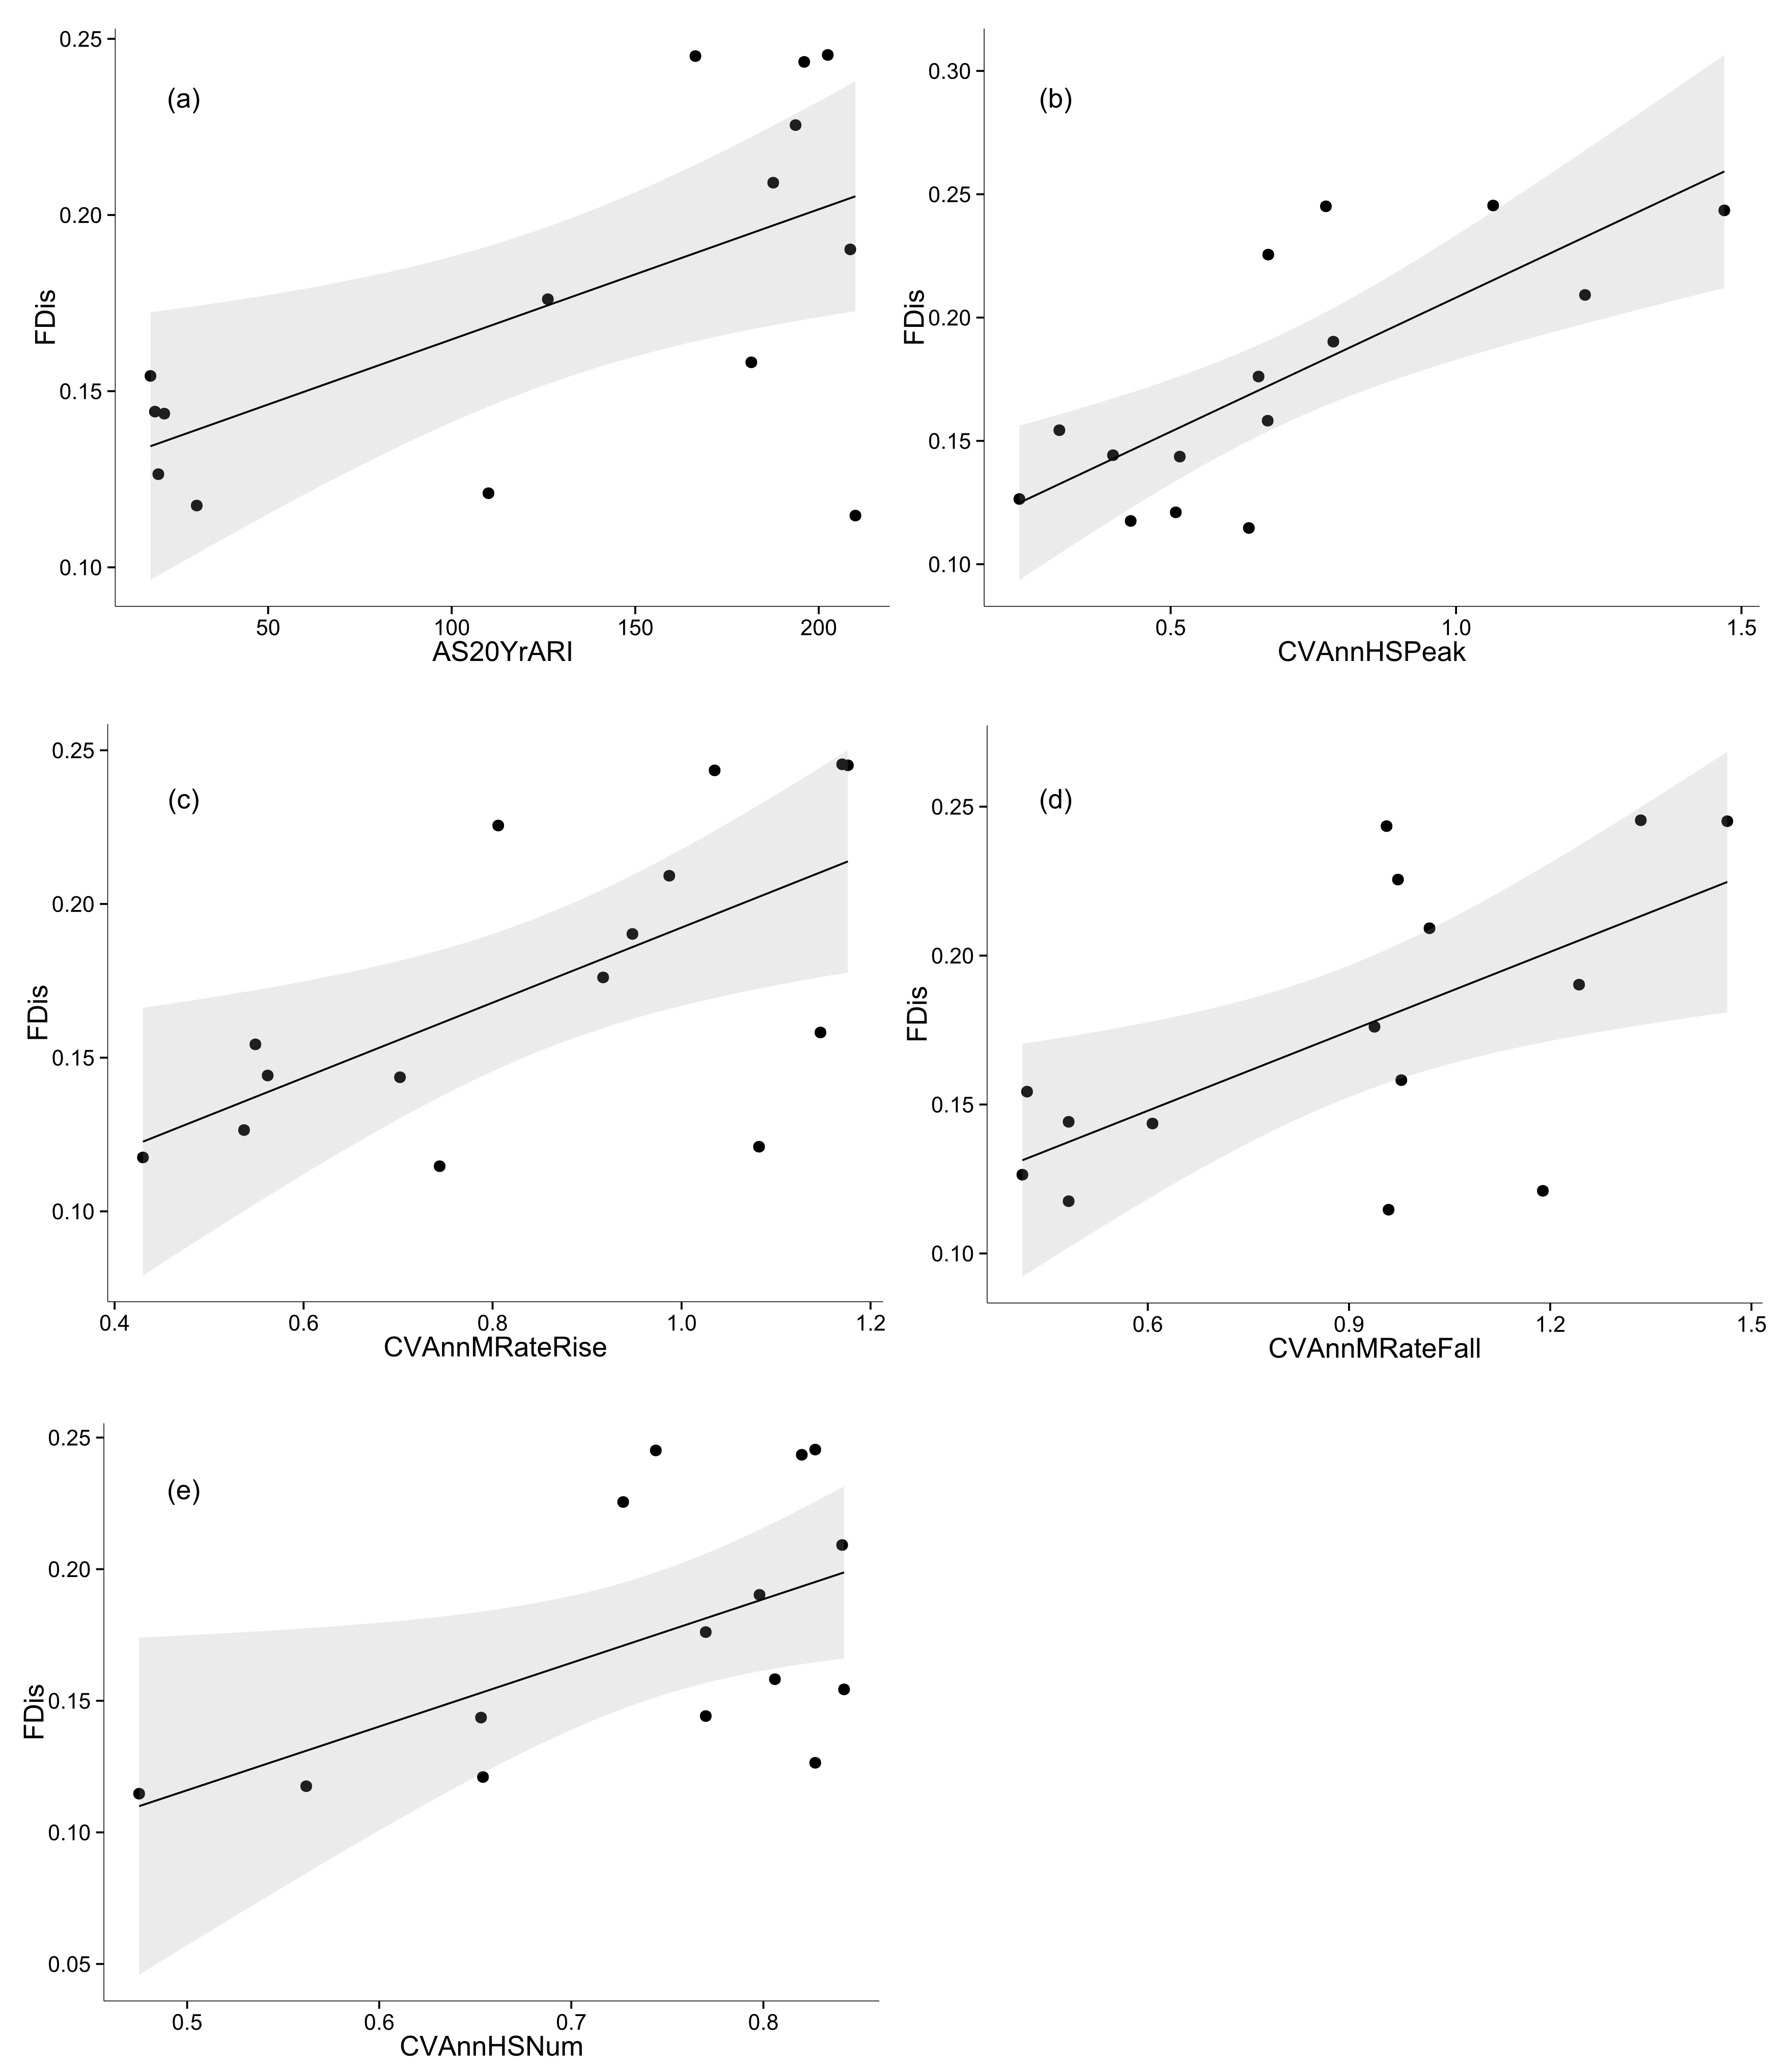
\includegraphics[width=\textwidth,keepaspectratio=true]{fig1.png} % figures can be in pdf, png, jpeg or eps format
\caption[Relationships between FDis and hydrological metrics describing flood magnitude.]{\small{Relationships between FDis and hydrological metrics describing (a) magnitude of the 20 year average return interval flood (AS20YrARI), (b) interannual variability in high flow magnitude (CVAnnHSPeak), (c) interannual variability in flood rise rate (CVAnnMRateRise), (d) interannual variability in flood fall rate (CVAnnMRateFall), (e) interannual variability in high flow frequency. Fitted lines depict ordinary least squares regression models. All models are linear fits. Shaded areas depict the smoothed 95 \% confidence interval around the regression model. All relationships shown are significant.  Units shown in Table 2.}}
\label{Ch3_F1} % label for cross-referencing
\end{center}
\end{figure}   
\clearpage

\subsection{Is functional diversity related to variability in seasonal water availability in the riparian zone?}
Functional dispersion was positively associated with variability in flow seasonality. FDis was increased when seasonal patterns of minimum (M\_MinM, Fig. 2a, adjusted p = 0.0278, R2 = 0.540), maximum (M\_MaxM, Fig. 2b, adjusted p = 0.0325, R2 = 0.328) and average (M\_MDFM, Fig. 2c, adjusted p = 0.0325, R2 = 0.347) flows became less uniform (smaller values of M) between years. In other words, at high FDis the season with which these flows were associated was not consistent through the record. FDis was not significantly explained by inter-seasonal uniformity of minimum (Fig. 2d, C\_MinM, adjusted p = 0.1021, R2 = 0.166) or average (Fig. 2e, C\_MDFM, adjusted p = 0.0861, R2 = 0.186) flows, although visual inspection of the scatterplots for these relationships indicates two sites at the lower bound of the x axis (i.e. strongly seasonal patterns of flow), with substantially lower FDis than predicted by the regression model. If we consider these trends, we can infer that functional dispersion was increased when discharge patterns differed strongly between seasons, but the season with which those patterns were associated was not consistent between years.

\begin{figure}[ht]
\begin{center}
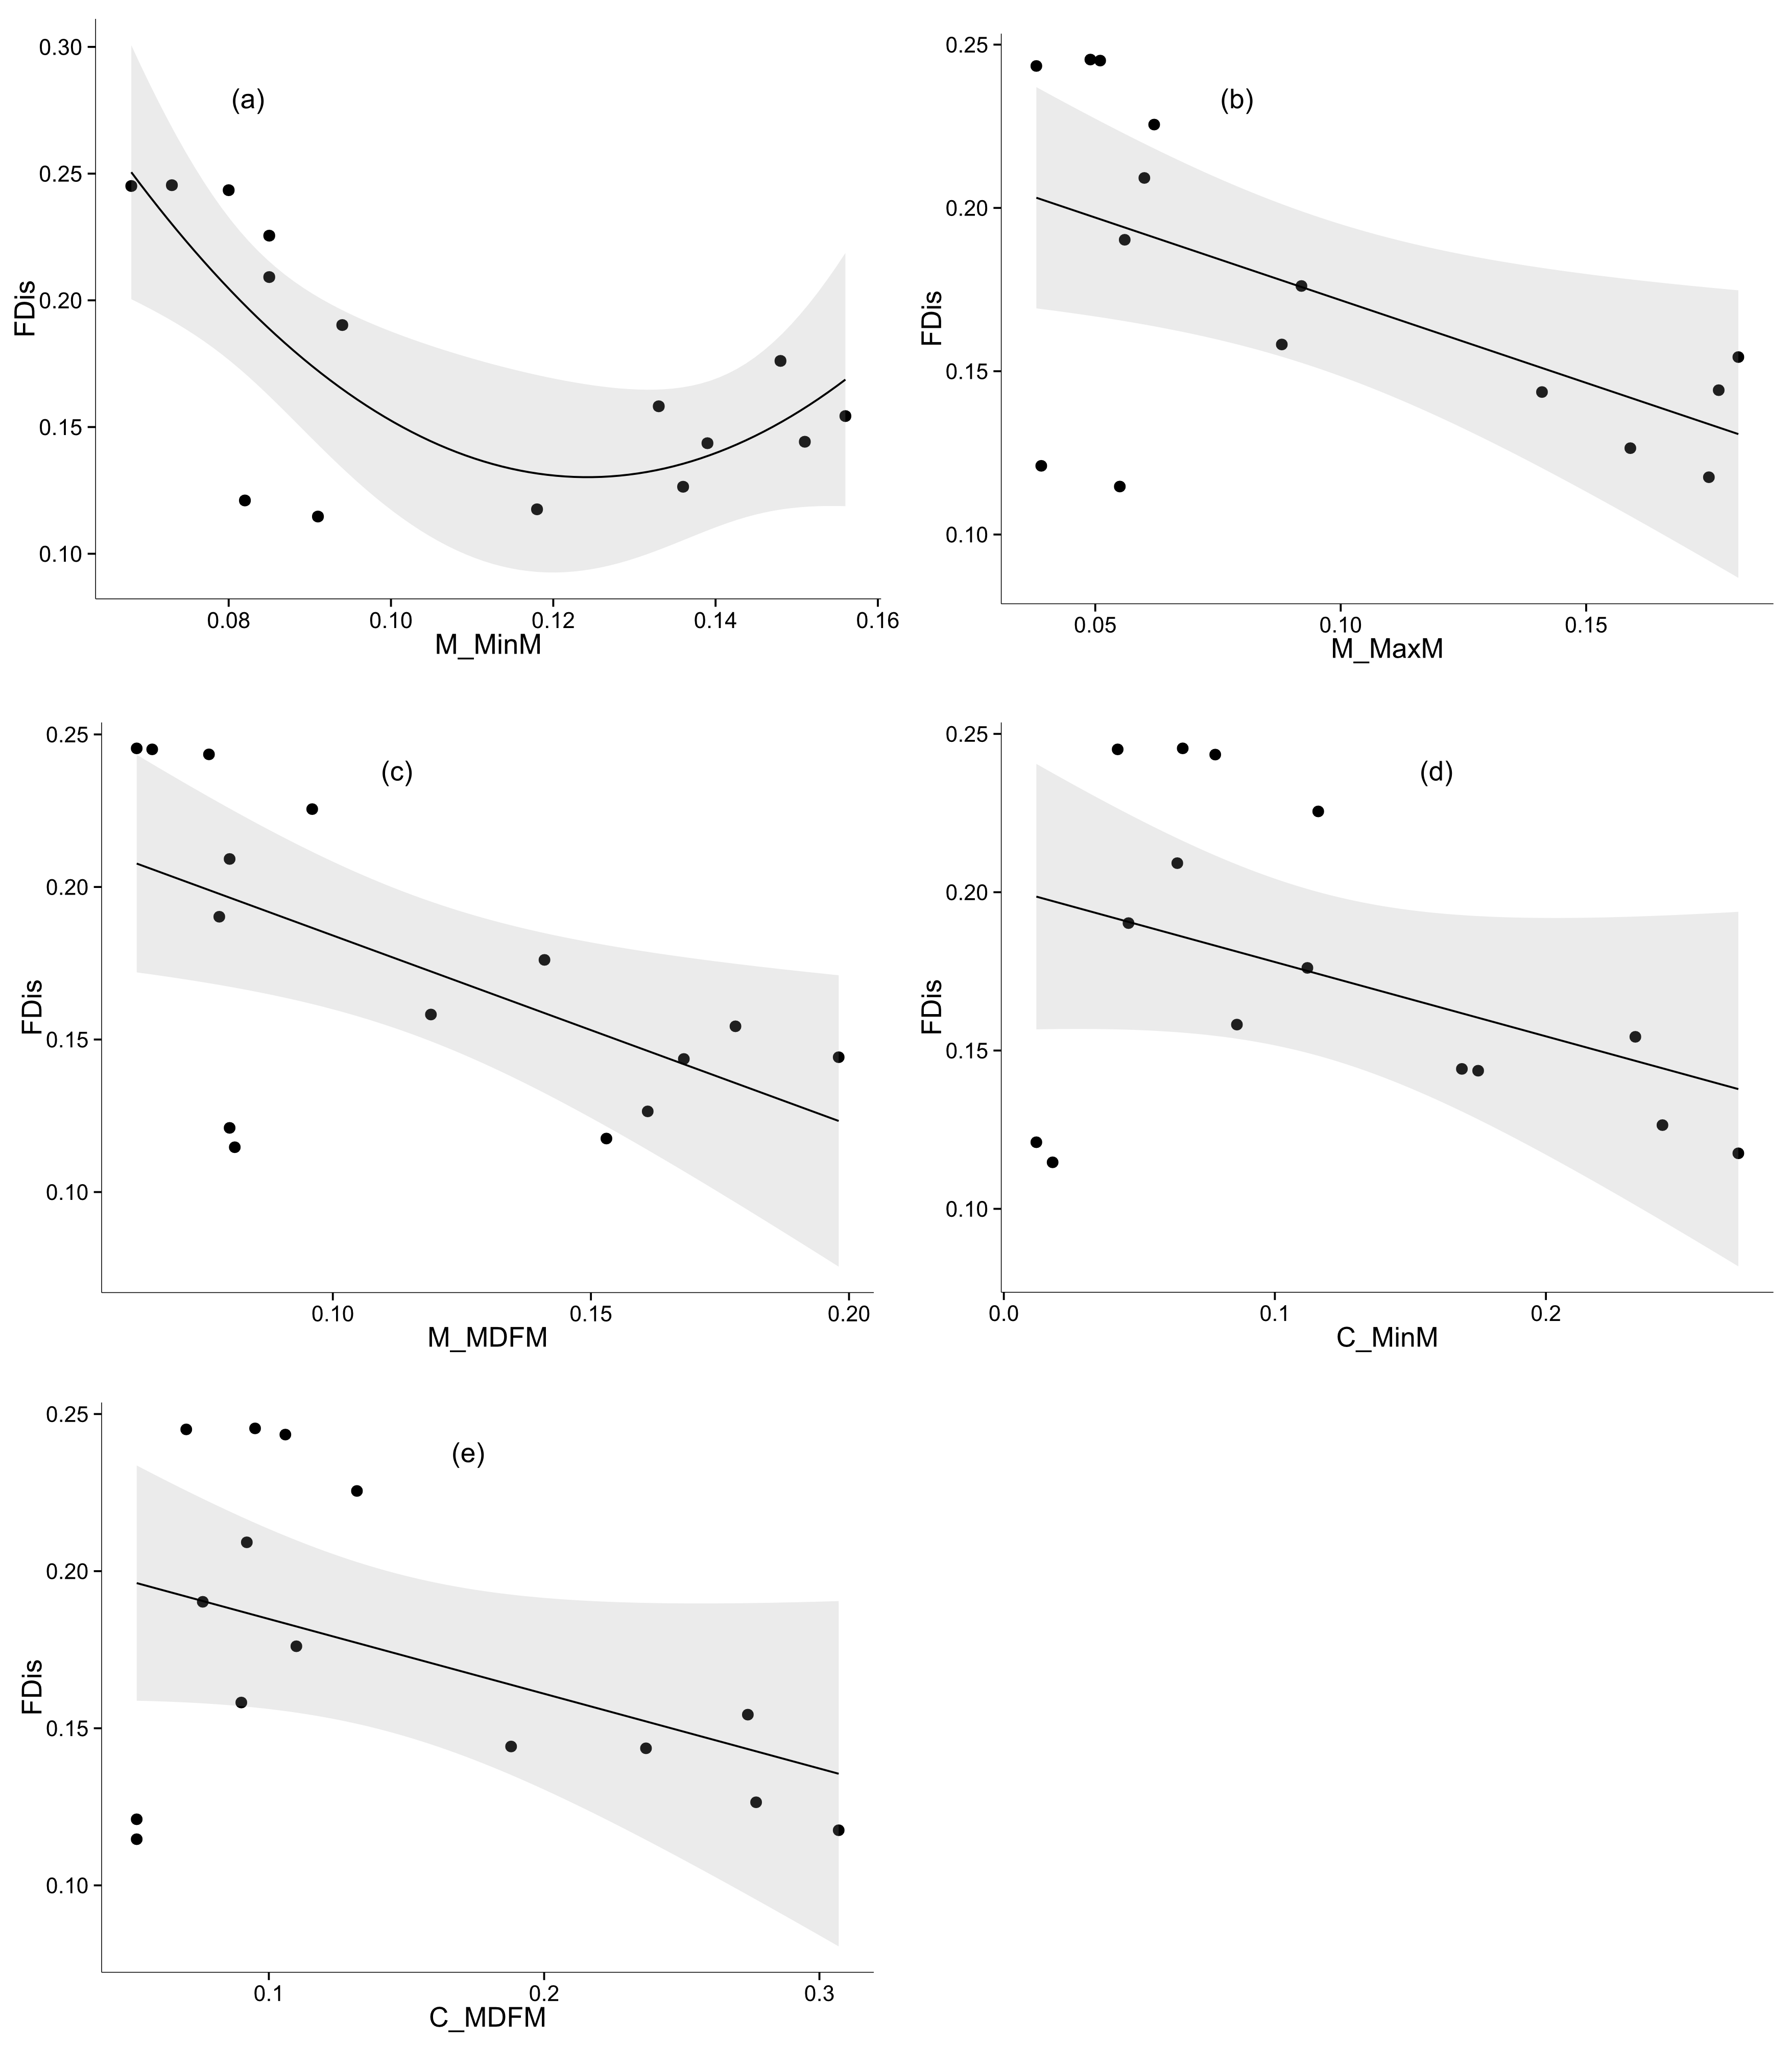
\includegraphics[width=\textwidth,keepaspectratio=true]{fig2.png} % figures can be in pdf, png, jpeg or eps format
\caption[Relationships between FDis and hydrological metrics describing variability in seasonal water availability (1).]{\small{Relationships between FDis and hydrological metrics describing (a) contingency of monthly minimum daily flow (M\_MinM), (b) contingency of monthly maximum daily flow (M\_MaxM), (c) contingency of monthly mean daily flow (M\_MDFM), (d) constancy of monthly minimum daily flow (C\_MinM), (e) constancy of monthly mean daily flow (C\_MDFM). Fitted lines depict ordinary least squares regression models. (a) is a quadratic fit, (b - e) are linear fits. Shaded areas depict the smoothed 95 \% confidence interval around the regression model. (a – c) depict significant relationships. (d - e) depict non-significant relationships (note the strong influence over the regression fit of the two points at the lower bound of FDis). Units are shown in Tables 1 and 2.}}
\label{Ch3_F2} % label for cross-referencing
\end{center}
\end{figure}   
\clearpage

This observation was corroborated by positive relationships between FDis and variability in mean daily flows for autumn (CVMDFAutumn, Fig. 3a, adjusted p = 0.0386, R2 = 0.301), winter (CVMDFWinter, Fig. 3b, adjusted p = 0.0278, R2 = 0.414) and spring (CVMDFSpring, Fig. 3c, adjusted p = 0.10325, R2 = 0.327). Summer flow variability (CVMDFSummer, Fig. 3d, adjusted p = 0.0325, R2 = 0.472) exhibited a humped relationship with FDis. Mean daily flows for both summer and spring were associated with FDis, however. This association was positive for summer (MDFMDF Summer, Fig. 3e, adjusted p = 0.0230, R2 = 0.503) and negative for spring (MDFMDFSpring, Fig. 3f, adjusted p = 0.0278, R2 = 0.3862).  Note that this metric actually represents the ratio of seasonal mean daily flow to the general mean of daily flow for a given river. Even though FDis was highest at sites where average flow is not associated with any particular season (low M\_MDFM), these sites still had high values for mean daily flow in summer. Pearson correlation confirms a significant negative relationship between M\_MDFM and MDFMDFSummer (Pearson’s r = -0.657, p = 0.008) but not C\_MDFM and MDFMDFSummer (Pearson’s r = -0.423, p = 0.1164). Summer mean daily flow may have been inflated by exceptional periods where very high average flows occurred during summer. Mean daily flow in spring, conversely, was strongly positively correlated with M\_MDFM (Pearson’s r = 0.8357, p = 0.0001) and C\_MDFM (Pearson’s r =0.7839, p = 0.0005), indicating that where mean daily flows in spring are high, this pattern is stable and consistent between years.

\begin{figure}[ht]
\begin{center}
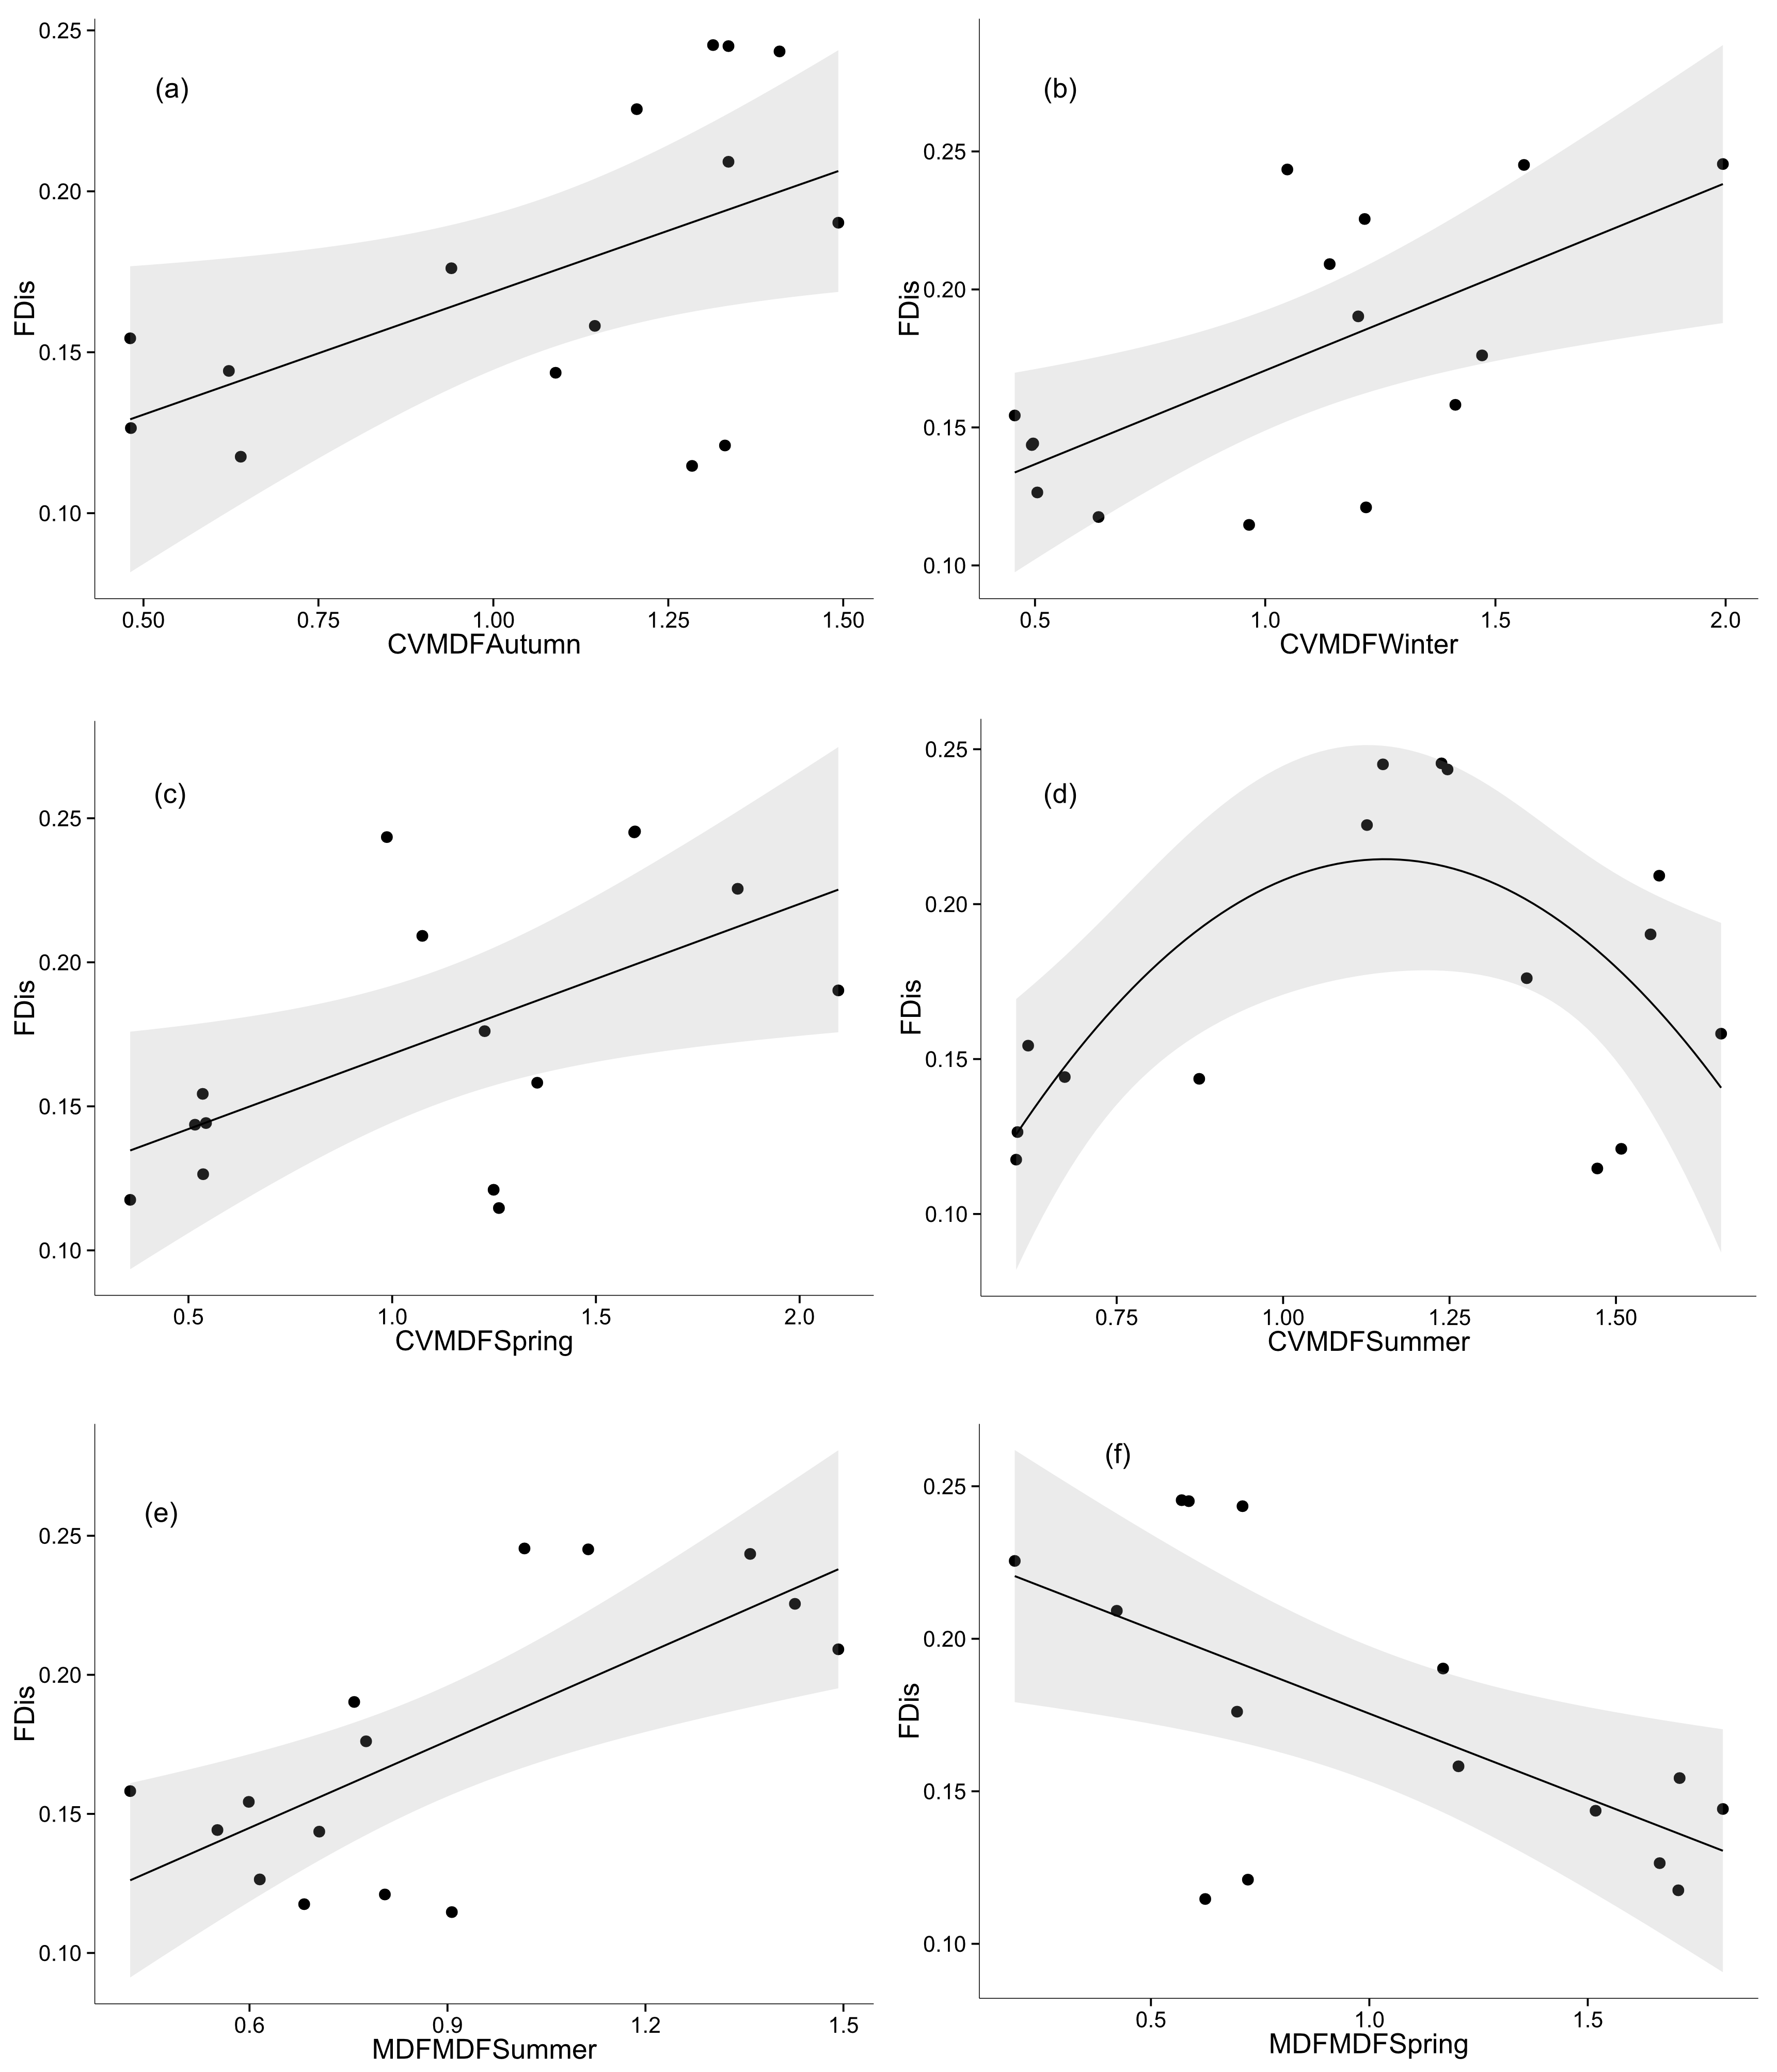
\includegraphics[width=\textwidth,keepaspectratio=true]{fig3.png} % figures can be in pdf, png, jpeg or eps format
\caption[Relationships between FDis and hydrological metrics describing variability in seasonal water availability (2).]{\small{Relationships between FDis and hydrological metrics describing (a) variability in autumn mean daily flow,(b) variability in winter mean daily flow, (c) variability in spring mean daily flow, (d) variability in summer mean daily flow, (e) mean daily flow in summer, (f) mean daily flow in spring. Fitted lines depict ordinary least squares regression models. All models are linear fits except in (d), which is a quadratic fit. Shaded areas depict the smoothed 95 \% confidence interval around the regression model.  All relationships shown are significant.  Units are shown in Tables 1 and 2.}}
\label{Ch3_F3} % label for cross-referencing
\end{center}
\end{figure}   
\clearpage


\subsection{Comparisons with measures of taxonomic diversity}
Across the species used in the functional diversity analysis (i.e. present at >1 \% plot cover), FDis was independent of species richness (p = 0.274, F(1,13) = 1.302) and Simpson’s diversity (p = 0.513, F(1,13) =  0.454) for species included in the functional diversity analysis, but significantly associated with species richness for the full set of 327 species (p = 0.030, F(1,13) = 5.957, R2 = 0.314).

\subsection{A minimal multiple regression model to explain functional diversity according to hydrology}
We used an information theoretic procedure to select the best fitting, most parsimonious multiple regression model from the factorial set of possible models which included FDis as the dependent variable and the following independent variables: interannual variability in high flow frequency (CVAnnHSNum), interannual variability in high flow magnitude (CVAnnHSPeak) and mean daily flow during summer (MDFMDFSummer). This set of models is described in Table 3.
\begin{landscape}
\begin{table}[ht]
\tiny
\centering
\caption[Multiple regression models with associated fitting parameters.]{\small{Multiple regression models with associated fitting parameters. * in the model formula denotes both summation as well as interaction between variables. R2 values have been adjusted for multiple regression for models using more than one variable. The optimal model according to AICc is indicated by bold typeface.}}
\label{Ch3_T3}
{\tabulinesep=1.2mm
\begin{tabu}to \linewidth {lp{12cm}XXX}
\hline
\textit{\#} & \textit{Model} & \textit{adj. R2} & \textit{AICc} & \textit{delta AIC} \\ \hline
1 & FDis {\raise.17ex\hbox{$\scriptstyle\mathtt{\sim}$}} CVAnnHSNum & 0.296 & -46.14 & 12.78 \\
2 & FDis {\raise.17ex\hbox{$\scriptstyle\mathtt{\sim}$}} CVAnnHSPeak & 0.577 & -53.79 & 5.13 \\
3 & FDis {\raise.17ex\hbox{$\scriptstyle\mathtt{\sim}$}} MDFMDFSummer & 0.503 & -51.37 & 7.56 \\
4 & FDis {\raise.17ex\hbox{$\scriptstyle\mathtt{\sim}$}} CVAnnHSNum + CVAnnHSPeak & 0.636 & -54.52 & 4.40 \\
5 & FDis {\raise.17ex\hbox{$\scriptstyle\mathtt{\sim}$}} CVAnnHSNum + MDFMDFSummer & 0.681 & -56.50 & 2.42 \\
6 & FDis {\raise.17ex\hbox{$\scriptstyle\mathtt{\sim}$}} CVAnnHSPeak + MDFMDFSummer & 0.561 & -51.71 & 7.21 \\
7 & FDis {\raise.17ex\hbox{$\scriptstyle\mathtt{\sim}$}} CVAnnHSNum * CVAnnHSPeak & 0.655 & -51.95 & 6.97 \\
8 & FDis {\raise.17ex\hbox{$\scriptstyle\mathtt{\sim}$}} CVAnnHSNum* MDFMDFSummer & 0.665 & -52.40 & 6.53 \\
9 & FDis {\raise.17ex\hbox{$\scriptstyle\mathtt{\sim}$}} CVAnnHSPeak * MDFMDFSummer & 0.566 & -48.54 & 10.39 \\
10 & FDis {\raise.17ex\hbox{$\scriptstyle\mathtt{\sim}$}} CVAnnHSNum + CVAnnHSPeak + MDFMDFSummer & 0.704 & -54.25 & 4.68 \\
11 & FDis {\raise.17ex\hbox{$\scriptstyle\mathtt{\sim}$}} CVAnnHSNum * CVAnnHSPeak + MDFMDFSummer & 0.709 & -50.14 & 8.79 \\
12 & \textbf{FDis {\raise.17ex\hbox{$\scriptstyle\mathtt{\sim}$}} CVAnnHSNum + CVAnnHSPeak * MDFMDFSummer} & 0.838 & -58.92 & 0 \\
13 & FDis {\raise.17ex\hbox{$\scriptstyle\mathtt{\sim}$}} CVAnnHSNum * CVAnnHSPeak * MDFMDFSummer & 0.944 & -48.62 & 10.30 \\ \\
\hline
\end{tabu}}
\end{table}
\end{landscape}

Model 12 was determined to be the optimal model according to AICc. Models 4, 5 and 10 were close to optimal but offered lower explanatory power according to the adjusted R2 of the model. Although Model 13 offered higher explanatory power, it was less parsimonious according to AICc and exhibited multicollinearity. Multicollinearity was determined not to be of importance for Model 12 according to variance inflation factor scores (all <3 on centred variables).  All terms in Model 12 were individually significant; a full summary of the model is given in Table 4. Notably, the coefficient of the interaction term was negative, indicating a diminishing influence on FDis when values of CVAnnHSPeak and MDFMDFSummer are both high.

\newpage

\begin{table}[ht]
\tiny
\centering
\caption[Regression summary for Model 12.]{\small{Regression summary for Model 12. Beta values are regression coefficents (B) standardised by the standard deviation of the term.}}
\label{Ch3_T4}
{\tabulinesep=1.2mm
\begin{tabu}to \textwidth {p{6cm}XXXXX}
\hline
& \textit{B} &	\textit{SE} &	\textit{beta} &	\textit{t}	 & \textit{p} \\
\hline
CVAnnHSNum	& 0.240 & 	0.054&	0.540&	4.414&	0.001 \\
CVAnnHSPeak&	0.071&	0.026&	0.498&	2.773&	0.020 \\
MDFMDFSummer&	0.074&	0.024&	0.506&	3.056&	0.012 \\
CVAnnHSPeak * MDFMDFSummer&	-0.190&	0.060&	-0.459&	-3.186&	0.001 \\ \\ \hline 
\end{tabu}}
\end{table}

\begin{table}[ht]
\tiny
\centering
\caption[Partioning of variance in FDis as explained by optimal hydrological and climatic models.]{\small{Partioning of variance in FDis as explained by optimal hydrological and climatic models. The ‘|’ symbol denotes ‘controlled for’; that is, variation explained non-redundantly by a fraction.}}
\label{Ch3_T5}
{\tabulinesep=1.2mm
\begin{tabu}to \textwidth {p{6cm}XX}
\hline
\textbf{Combined fractions:}	& \textit{df}&	\textit{adjusted R2} \\
a + b (hydrology)&	4&	0.838 \\
b + c (climate)&	2&	0.629\\
a + b + c (hydrology + climate)&	6&	0.854\\
\hline
\textbf{Individual fractions:}& & 		\\
a (hydrology | climate)&	4&	0.226\\
b (shared variation)&	0&	0.612\\
c (climate | hydrology)&	2&	0.016\\
d (unexplained variation)& &		0.46\\
\hline
\end{tabu}}
\end{table}
\clearpage

\subsection{Do climatic or edaphic conditions explain variation in FDis that is unaccounted for by hydrological metrics?}
Of the 19 climatic variables examined, a number exhibited statistically significant univariate relationships with FDis; the quadratic function of isothermality was determined by AICc to be the optimal regression model. Of the 12 edaphic variables examined, no significant univariate relationships with FDis were found.  Variance partitioning showed that while the dominant fraction of variation explained by the two models was shared (0.612), the climatic model explained a minimal amount of non-redundant information (0.016) compared with the hydrological model (0.226), indicating a dominant influence of hydrological flow regime on functional dispersion in this study. Table 5 shows the partition table generated from this analysis.



\section{Discussion}
We surveyed vegetation communities along partly confined river systems across south-eastern Australia and found that functional diversity, as characterised by functional dispersion, exhibited strong relationships with local patterns of hydrology. To our knowledge this is the first study to examine relationships between hydrological conditions and the diversity of ecological strategies within riparian vegetation communities using multiple quantitative functional traits. The overarching pattern across these relationships can be summarised as “heterogeneous flows foster heterogeneous communities”.

This pattern is consistent with existing understanding of the processes that generate and maintain biological diversity in the riparian environment. Briefly stated, this paradigm holds that riparian biodiversity is a function of landscape complexity generated by hydrogeomorphic processes, overlain by feedback interactions between these processes and biotic components of the riparian environment \cite{Tabacchi1996, Palmer1997, Corenblit2007, Bornette2008}(Tabacchi et al. 1996; Palmer & Poff 1997; Corenblit et al. 2007; Bornette et al. 2008}. Because we surveyed geomorphically homogeneous sections of sloping bank, our argument is presented under the assumption that functional diversity is a property of riparian communities at the reach scale. Influx of species from more physically complex adjacent patches, then, is responsible for the diversity we observed on these geomorphologically homogeneous sloping bank sections.

The sites surveyed in this study spanned a spectrum of flooding intensity: the 20-year average return interval (ARI) flood ranged from 18 times the mean daily flow to 210 times the mean daily flow. Higher magnitude flow events are more likely to be geomorphically effective in partly confined river systems \cite{Huang2006}. The strong positive relationship between functional diversity and 20-year ARI flood magnitude supports the supposition that disturbance retards competitive exclusion as a diversity limiting process \textit{sensu} \cite{Huston1979}. Notably, no significant relationships were found between functional diversity and metrics describing mean high flow conditions, whereas metrics describing variability had high explanatory power. Interannual variability in high flow magnitude showed the strongest relationship with functional diversity in this study. If a causal relationship exists, it could be because the average high flow magnitude determines what proportion (in terms of elevation above the main channel) of the riparian zone experiences flooding in a given year. Variability in high flow magnitude, combined with geomorphic heterogeneity, will produce variability in the time since last inundation (without significant disturbance), or combined inundation and disturbance, for a given patch of vegetation. Since flood flows also function as an important dispersal pathway for propagules \cite{Merritt2010a}, variability in high flow magnitude should influence recruitment processes in a similar manner.  Likewise, variability in the frequency of flood flows also results in variable time since last inundation or disturbance. Interannual variability in flood rise and fall rates was also positively associated with functional diversity. Overall, the combination of occasional high intensity flooding disturbance with year-to-year variability in patterning of high flow events results in a heterogeneous patch mosaic. This environmental heterogeneity provides a broad range of niches, facilitating the success of a diversity of ecological strategies \cite{Bornette2008}.
 
We can extend this framework to account for the observed relationships between functional diversity and variability in seasonal water availability.  Our sites spanned a gradient of flow seasonality: at one end, rivers exhibited weak but stable patterns of seasonality; at the other, rivers were characterised by high interannual variability and modal, seasonally inconsistent distributions of flow. Once again, communities with higher functional diversity tended to be located towards the ‘variable’ end of the spectrum. South-eastern Australian plants do exhibit characteristic species-level responses to seasonality, although there is no general coordination of growth and reproduction phenologies as in the northern hemisphere \cite{Ford1979}. Flowering times within the Myrtaceae (a dominant family in riparian plant communities of south-eastern Australia) are often staggered where species are sympatric \cite{Beardsell1993}, and growth and reproduction of riparian plants are commonly associated with the arrival of favourable conditions \cite{Woolfrey2001, Robertson2001, Seibentritt2004}. High coefficients of variation in seasonal mean daily flows may therefore act to temporarily provide species with favourable conditions according to their seasonal biology.
 
Exceptions to these patterns included the quadratic fit for variability in summer mean daily flows, with high values being associated with a reduction in functional diversity, and mean daily flow for summer, which was positively associated with functional diversity and broke the trend of associations with seasonal means being either non-significant or negative. A meta-analysis of the effect of drought on riparian vegetation showed reduced species richness and a shift towards drought-tolerant species following climate-induced increases in the intensity and duration of drought, an effect that was exacerbated by high temperatures \cite{Garssen2014}. Higher temperatures in the absence of drought were associated with higher rates of primary production. Higher mean daily flows in summer, then, potentially alleviate the water stress induced by hot weather while stimulating plant growth. We did investigate whether sites at subtropical latitudes simply had higher functional diversity than temperate sites, according to well-known latitudinal patterns of species richness \cite{Willig2003}, and found no relationship between latitude and FDis (data not presented). 

It was notable that while FDis is statistically independent of species richness, in this study functional dispersion was significantly associated with total species richness (as opposed to richness of the set of species used in the FDis analysis that were present at >1 \% abundance). A broad species pool therefore appears to facilitate higher functional dispersion within the dominant flora of a community, even though the richness of the dominant group of species does not necessarily determine functional diversity. It is difficult to interpret this finding, however, as adding data for rare species to the analysis would necessarily render the new value of FDis independent of total species richness.

The multiple regression model selected according to AICc explained a high proportion of variation in FDis. This model described functional diversity as a function of variability in flood frequency and magnitude, and in summer mean daily flow. The combination of flow heterogeneity with extra watering during summer appears to provide optimal conditions for functionally diverse communities. The coefficient of the interaction term between variability in flood magnitude and summer mean daily flow was significant but negative, indicating that the additive effect is subject to diminishing returns at high values of both terms. The key finding here is that these three metrics of hydrological conditions are able to account for most of the variation in FDis; data on climatic conditions and edaphic properties add very little non-redundant information to our model. We used traits in our analysis that capture a broad spectrum of ecological strategies, rather than solely traits associated with riparian specialist strategies, which might be expected to bias results towards flow response. We caveat, however, that this model does not account for the effect of plot-scale geomorphic variability on diversity, as this was controlled for in the site selection process.
 
Two sites had anomalous values for FDis that do not fit within this conceptual model of disturbance and flow variability providing high niche heterogeneity. These sites experience highly variable flows but had low functional diversity. We experimentally adjusted the abundances of dominant species at these sites and found that the low values for FDis appear to result from dominance of a single species at each site (the medium sized tree \textit{Acmena smithii} at Mammy Johnson’s Creek, and the liana \textit{Ripogonum album} at Jilliby Creek). These sites may represent cases in which species with ‘variability’ specialist strategies have become dominant. \textit{Acmena smithii} has a relatively large seed and is shade tolerant \cite{Melick1990}, but once established, develops a lignotuber and is highly resistant to drought and disturbance \cite{Ashton1976}. With respect to \textit{Ripogonum album}, there is evidence to suggest that abundance of lianas may be associated with disturbance \cite{Laurance2001} and that lianas have a competitive advantage over trees in dry conditions \cite{Swaine2007, Cai2009}, but see \cite{Nepstad2007}.
 
Our survey covered approximately half of the range of hydrological variability present within the Australian continent; much of the lower range and middle range was captured, but highly variable dryland systems were not included \cite{Peel2004}. Our results mostly show monotonic relationships between FDis and hydrological heterogeneity, and as such do not support intermediate disturbance associated patterns found in other studies of taxonomic \cite{Bendix1997, Bendix2000, Lite2005, Corenblit2007} and functional diversity \cite{Biswas2010} of riparian plant communities. This finding is consistent with the assertion of \cite{Mouillot2013} that metrics of functional diversity should show monotonic rather than unimodal relationships with disturbance intensity. It is difficult to be conclusive on this point, however, as it is possible that we have found only the ascending half of a unimodal curve. To this end, it would be useful to survey communities that experience more extreme hydrologies, such as those in Australia’s arid regions or the monsoon tropics. Disturbance intensity and hydrological heterogeneity may not necessarily be connected in such systems. Arid zone rivers characterised by ‘all or nothing’ flow regimes may not experience the moderate flood events that generate and maintain diversity at the patch scale; for monsoonal rivers, disturbance may be similarly intense, but seasonal and interannual patterns of flow are relatively predictable \cite{Kennard2010}. In large tropical riverscapes, hydrological rhymthicity (i.e. the opposite of hydrological heterogeneity) has in fact been associated with greater richness of fish and bird taxa, and greater production in riparian forests \cite{Jardine2015}.

Unlike anthropogenic disturbances associated with agricultural land use, which have been shown to be associated with lower functional richness \cite{Pakeman2011} and lower functional redundancy \cite{Laliberte2010}, recurring hydrological disturbance appears to promote riparian plant functional diversity in this study. A similar response to natural fire regimes in the Patagonian steppe has also been observed \cite{Sottile2015}. It seems reasonable to assume that the generative effect of natural disturbance on niche heterogeneity is not reproduced by typical anthropogenic disturbances.
 
Our findings are important from an applied river management and conservation perspective. Widespread anthropogenic river modification has altered the hydrology of river systems throughout the world, and the changing climate has the potential to exacerbate the impacts of flow modification as well as affecting unaltered river systems. A key issue with river modification is that it reduces flow heterogeneity. Dams flatten flood hydrographs (and peaks), alter seasonality and increase predictability of flows \cite{Graf2006, Singer2007}. These alterations to flow have ‘terrestrialised’ riparian areas and wetlands, reducing functional diversity and facilitating invasion by exotic terrestrial weed species \cite{Catford2011}.  Dams also interrupt hydrochorous transport of propagules \cite{Merritt2010a}, such that flood flows below dams may cause net removal of propagule material from fluvial substrates, rather than deposition. When designing environmental flows (e.g. \cite{Howell2000}), river managers typically consider magnitude, frequency and seasonality of flows. The findings in this paper agree with recent suggestions \cite{Naiman2008} that managers should also attempt to simulate flow regime variability in their designed flows.
 
Future runoff predictions are regionally specific but similarly include changes to total discharge, flow seasonality and flow variability. In regions with projected increases in climatic variability, changes to the prevalence, intensity and timing of extreme flooding or drought events can be expected \cite{Hennessy2008}. Reductions in mean summer precipitation have already occurred over large areas of Australia, coinciding with a warming of 0.4 – 0.7 oC since 1950 \cite{Hennessy2007}. Lower average flows during hotter summers may stress riparian communities and constrain functional dispersion. Alternatively, greater climatic variability associated with future climates \cite{Hennessy2008} may promote hydrological heterogeneity in regions that were previously associated with more stable flow conditions. This may result in opening of niche space to favour opportunistic ecological strategies and promote invasion by exotic species.
 
Restoring functional diversity to pre-degradation levels may be a useful goal for riparian rehabilitation efforts along regulated or otherwise degraded river reaches. High functional diversity communities encompass a broad range of ecological strategies and should have a greater capacity to adapt to environmental change \cite{Tilman1997, Standish2014}. By working to restore functional diversity along impacted river systems, managers may increase the likelihood that riparian communities will be able to maintain critical ecosystem functions under future climates.
 
The identification of such a strong relationship between environmental variability and functional diversity has significance for lotic ecology \cite{Palmer1997}, as well as ecology in general. Our study emphasises the importance of flooding disturbance and hydrological heterogeneity as drivers of functional diversity in riparian plant communities. These findings should be applicable to river systems in other regions and biomes characterised by moderate hydrological variability, given the profound influence of hydrology in shaping the structure of fluvial landscapes and determining the ecological strategies of plants that are able to persist and thrive in the riparian environment. Comparisons with datasets from regions with harsh but highly predictable seasonal patterns of hydrology, for example monsoonal or nival regimes, are needed to confirm this assertion. In the south-eastern Australian context, at least, alterations to flow variability and disturbance regimes by dams and the changing climate may have significant consequences for the diversity and functioning of riparian vegetation communities.

\section*{Acknowledgements}
Saskia Grootemaat, Ashley Vey, Urvashi Lallu, Julia Atkinson, Sally Lawson and Anthony Manea assisted in the field. We also wish to thank the New South Wales Parks and Wildlife Service and Parks Victoria and their dedicated officers who provided logistical advice and support. Thanks also to the landowners who were kind enough to let us work on their properties and invited us into their homes. The insight of two anonymous reviewers and suggestions the Associate Editor of Freshwater Biology, Colin Townsend, helped us to improve our draft manuscript. This research was supported by Macquarie University and an Australian Postgraduate Award scholarship to James Lawson.

\section*{Data availability}
Trait data for all species are available at \url{http://onlinelibrary.wiley.com/doi/10.1111/fwb.12649/suppinfo}.

%%%%% REFERENCES % this is in a new chapter due to the memoir format
\renewcommand\bibname{{References}} 
\begin{small}
\bibliographystyle{apalike}
\bibliography{library}
\end{small}

\end{document}



